% Template create by Ariel Soto-Caro, Jan-2019.
% asotocaro@ufl.edu & arielsotocaro@gmail.com
% This template is availible at github as well:
% https://github.com/ArielSotoCaro/FRED_beamer_theme/
\documentclass[aspectratio=169]{beamer}
\usepackage{UFtheme}
\usepackage{multicol}
\setbeamertemplate{caption}[numbered]
\setbeamertemplate{bibliography item}{\insertbiblabel}
\usepackage{multirow}



%% ===========================================
%% ===========================================
\title{\huge Classification of Stars using Stellar Spectra collected by the Sloan Digital Sky Survey}
\author{Michael Brice and R\u{a}zvan Andonie}
\institute{Computer Science Department: Central Washington University}
\date{July 16, 2019}


%% ===========================================
%% ===========================================
\begin{document}


\begin{frame}[plain]
    \titlepage
\end{frame}
%% ===========================================
%% ===========================================

% Uncomment these lines for an automatically generated outline.
\begin{frame}{Outline}
\begin{multicols}{2}
  \tableofcontents
\end{multicols}
\end{frame}


%% ===========================================
%% ===========================================
\section{Introduction} 

\begin{frame}
\frametitle{Introduction}
. 
\begin{itemize}
	\item Avoids complex transformation and statistical analysis of the spectra space.
	\item Use spectra without redshift corrections.
	\item Use Machine Learning classifiers.
	\item Uses Standard Feature Selection Methods to reduce the number of flux measurements.
\end{itemize} 

\end{frame}


%% ===========================================
%% ===========================================
\section{Astronomy Background}
\begin{frame}
\frametitle{}

\begin{center}
\LARGE
Astronomy Background
\end{center}

\end{frame}

\subsection{Stellar Spectra}

\begin{frame}
\frametitle{Stellar Spectra}

  \begin{block}

    \begin{columns}[t]

      \column{.5\textwidth} % Left column and width
\vspace{-1cm} 
	\begin{itemize}
	\item A \textit{spectrum} (plural \textit{spectra}) is defined as the way in which light is distributed with wavelength \cite{Chromey}. 

	\item Incandescent light bulbs, when viewed with the unaided eye, appears to emit white light, but when viewed through a prism or a diffraction grating, the bulb is actually emitting a rainbow or spectrum of light. Stellar spectra work the same way. 
	\item Unlike the example with the incandescent light bulb, stellar spectra have interesting properties. 
	\end{itemize}
      \column{.45\textwidth} % Right column and width
        \begin{figure}[T]
	 \vspace{-1cm} 
            \centering
            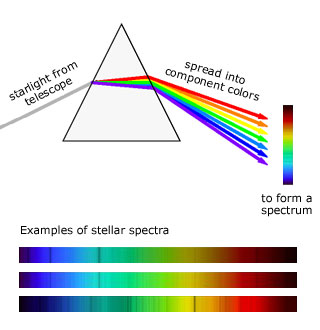
\includegraphics[width=2.0in]{spectrum.jpg}
            \caption{A spectrum \cite{spectrum}.}
            \label{fig:spectrum}
        \end{figure}

    \end{columns}
  \end{block}

\end{frame}

\begin{frame}
\frametitle{Stellar Spectra}

  \begin{block}

    \begin{columns}[t]

      \column{.5\textwidth} % Left column and width
\vspace{-1cm} 
	\begin{itemize}
	\item Stellar spectra contain wavelength measurements and flux measurements. 
	\item \textit{Wavelengths} are discrete values that represent a range of wavelengths of light. For example, a wavelength value can be 6,000$\pm5$ $\mathring{A}ngstr\ddot{o}ms$ ($\mathring{A}$).
	\item  \textit{Flux measurements} are the number of photons that pass through an area per second per measured wavelength. 
\item Fig. \ref{fig:G2} shows an example spectrum of a flux scaled G2 (Sun like) star. The downward spikes seen in Fig. \ref{fig:G2} are absorption lines.
	\end{itemize}
      \column{.45\textwidth} % Right column and width
        \begin{figure}[T]
	 \vspace{-1cm} 
	\hspace*{-.5cm} 
            \centering
            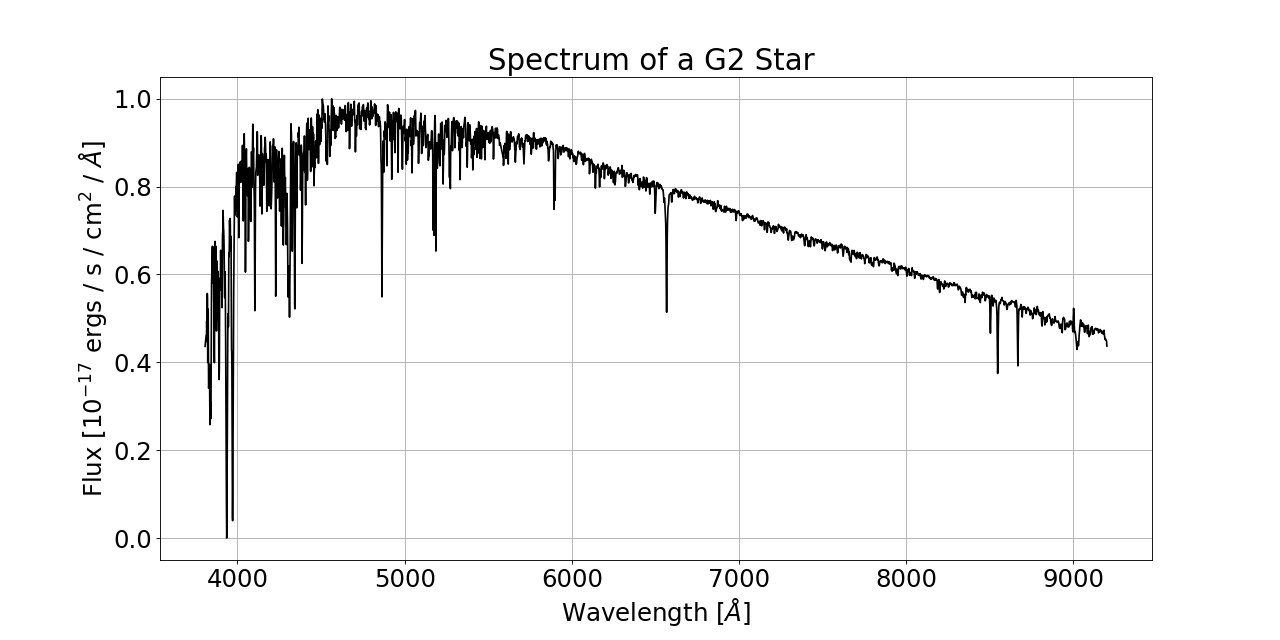
\includegraphics[width = 2.9in]{G2.png}
            \caption{Example: Stellar Spectrum of a flux scaled G2 star collected by the SDSS.}
            \label{fig:G2}
        \end{figure}

    \end{columns}
  \end{block}

\end{frame}

\subsection{Stellar Classification Types}
\begin{frame}
\frametitle{Stellar Classification Types}

\begin{itemize}
\item Two types of stellar classification schemes: The Harvard spectral classification and the Morgan - Keenan Luminosity Classes (MK) \cite{Carroll}.
\item The Harvard spectral classification is a surface temperature classification utilizing absorption lines
	\begin{itemize}
		\item O, B, A, F, G, K, and M
		\item Subclasses 0 - 9
	\end{itemize}
\item MK Luminosity Classes extends on the Harvard classes by adding a luminosity class and using the widths of the absorption lines.
	\begin{itemize}
		\item I, II, III, IV, V, VI
		\item Super Giants, Bright Giants, Sub-Giants, Main Sequence (Dwarfs), and Sub-Dwarfs \cite{Carroll}.
	\end{itemize}
\item For example, Betelgeuse is a red super giant and a stellar class of M1 (Harvard) Ia (MK) star and Proxima Centauri is a main sequence red dwarf and a stellar class of M6 V star. 
\end{itemize}

\end{frame}

\subsection{Importance of Stellar Classes}
\begin{frame}
\frametitle{Importance of Stellar Classes}
  \begin{block}

    \begin{columns}[t]
      \column{.45\textwidth} % Left column and width
\vspace{-0.5cm}
	\begin{itemize}
	\item Astronomers use stellar classes, in conjunction with other data, to learn many details about stars. 
\item The Hertzsprung-Russell (H-R) diagram, shown in Fig. \ref{fig:HR}, is a plot of stars where the horizontal axis is the spectral class or surface temperature and the vertical axis is the luminosity or absolute magnitude.
	\item The location of a star on the H-R diagram tells astronomers information about that star.\cite{Carroll}.
	\end{itemize}
      \column{.45\textwidth} % Right column and width
        \begin{figure}
	\vspace{-1cm} 
            \centering
            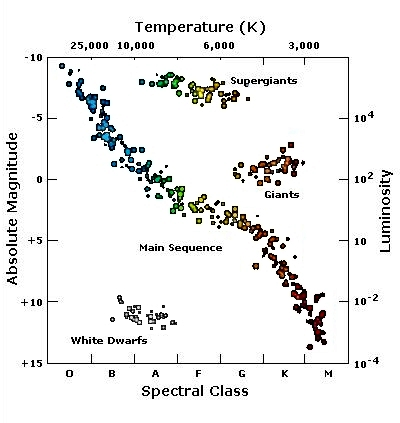
\includegraphics[scale = .37]{HR.jpg} %51
            \caption{Hertzsprung Russell Diagram \cite{hr}}
            \label{fig:HR}
        \end{figure}

    \end{columns}
  \end{block}

\end{frame}

\subsection{Redshift}
\begin{frame}
\frametitle{Redshift I}
  \begin{block}

    \begin{columns}[t]
      \column{.45\textwidth} % Left column and width
        \begin{figure}
	\vspace{-1cm} 
            \centering
            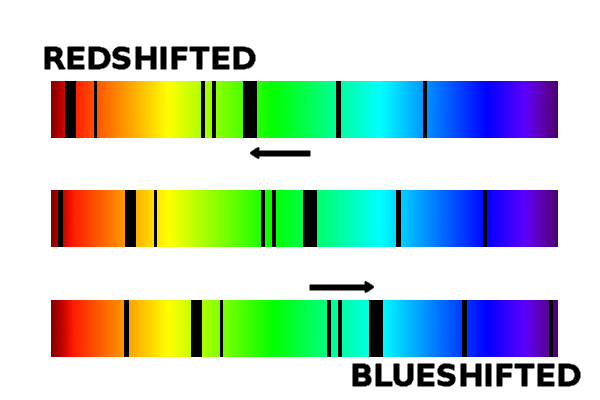
\includegraphics[scale = .32]{red2.png} %51
            \caption{Example of Redshift \cite{redshift}}
            \label{fig:red}
        \end{figure}

      \column{.45\textwidth} % Right column and width
        \begin{figure}
 
	\vspace{-0.5cm}
	\hspace*{-.5cm} 
            \centering
            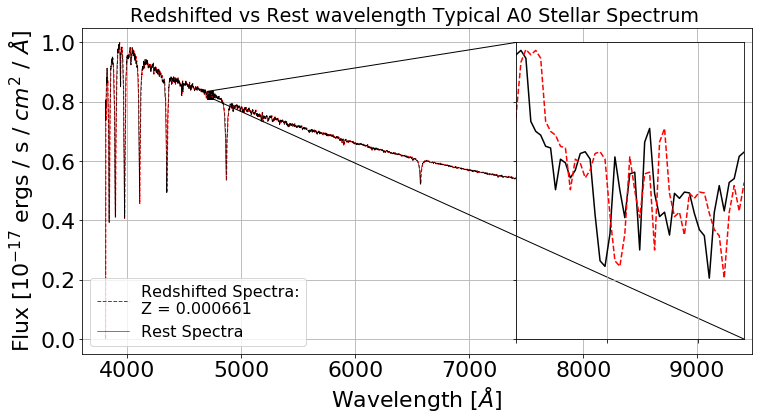
\includegraphics[width = 2.9in]{redshift.png} %51
            \caption{Another example of Redshift.}
            \label{fig:redshift}
        \end{figure}

    \end{columns}
  \end{block}
\end{frame}

\begin{frame}
\frametitle{Redshift II}
  \begin{block}

    \begin{columns}[t]
      \column{.45\textwidth} % Left column and width
\vspace{-0.5cm}
	\begin{itemize}
	\item Redshift is defined by (\ref{eq:red}), where \textit{Z} is the redshift value and $\lambda$ is the wavelength \cite{Carroll, Chromey}. 
	\item Equation (\ref{eq:flux1})  defines how the flux density changes due to redshift, where \textit{f} is the flux density at wavelength $\lambda$ (see \cite{Chromey}). 
	\item However, for the purpose of this thesis, since \textit{Z} for stars from the SDSS database have \textit{Z} $\ll$ 1, (\ref{eq:flux2}) is used.

	\end{itemize}
      \column{.45\textwidth} % Right column and width
               % Redshift equation
        \begin{equation}\label{eq:red}
            Z = \frac{\lambda_{observed} - \lambda_{rest}}{\lambda_{rest}}
        \end{equation}

	% Flux Redshift equation
        \begin{equation}\label{eq:flux1}
            f(\lambda_{rest}) = (1 + Z)^2 f(\lambda_{observed}) 
        \end{equation}

	% Flux Redshift equation
        \begin{equation}\label{eq:flux2}
            f(\lambda_{rest}) \approx f(\lambda_{observed})
        \end{equation}


    \end{columns}
  \end{block}

\end{frame}

\begin{frame}
\frametitle{Redshift III}

\vspace{-0.5cm}
	Human Redshift Extraction
	\begin{enumerate}
	\item Obtain the spectrum of a star which shows Absorption Lines.
	\item From the pattern of lines, identify which line corresponds to which atom, ion, or molecule.
		\begin{itemize}
		\item This pattern of lines are used to classify into the Harvard Spectral and Morgan Keenan Luminosity Classes.
		\end{itemize}
	\item Measure the shift of any one of those lines with respect to its expected wavelength, as measured in a laboratory on Earth.
	\item Apply a formula that relates the observed shift to velocity along the line-of-sight (eq. (\ref{eq:red}))
	\end{enumerate}


\end{frame}



% ======================================================================
\section{Data Source}

\begin{frame}
\frametitle{}

\begin{center}
\LARGE
Data Source
\end{center}
\end{frame}

%% ===========================================
%% ===========================================
\subsection{Sloan Digital Sky Survey}
\begin{frame}
\frametitle{Sloan Digital Sky Survey (SDSS)}
. 
  \begin{block}

    \begin{columns}[t]
      \column{.45\textwidth} % Left column and width
	\vspace{-1cm} 
	\begin{itemize}
	\item The SDSS has created the most detailed three-dimensional maps of the Universe ever made, with deep multi-color images of one third of the sky, and spectra for more than three million astronomical objects \cite{sdss}.
	\end{itemize}

      \column{.45\textwidth} % Right column and width
Bolton \textit{et al.} \cite{Bolton}

\begin{enumerate}

\item Uses templates.
\item Overall best fit (in terms of lowest reduced chi-squared) is used as classification.

\end{enumerate}

    \end{columns}
  \end{block}

\end{frame}

\begin{frame}
\frametitle{SDSS Data Pre-processing}
\begin{itemize}
\item The data is pre-processed by SDSS scientists through the methods presented by Dawson \textit{et al. }\cite{Dawson} and Stoughton \textit{et al.}  \cite{Stoughton}.
\item Two spectrographs used by the SDSS to collect the stellar spectra: the Baryon Oscillation Spectroscopic Survey (BOSS) spectrograph and the SDSS spectrograph described in Smee \textit{et al.} \cite{Smee}.  
\end{itemize}
\end{frame}

% ======================================================================
\section{The Approach}

\begin{frame}
\frametitle{}

\begin{center}
\LARGE
Classification into the Harvard Spectral Classification Scheme
\end{center}

\end{frame}

\subsection{Introduction}
\begin{frame}
\frametitle{Introduction}
\begin{itemize}
	\item Avoid complex transformation and statistical analysis of the spectra space.
	\item Spectra without redshift corrections.
	\item Use feature selection to reduce the number of flux measurements. Feature selection may destroy the shape and the structure of each stellar spectrum by only using the most relevant flux measurements. 
	\item Classifies only into the Harvard Spectral Classification Scheme.
\end{itemize}
\end{frame}

\subsection{Related Work}

\begin{frame}
\frametitle{Related Work I}
Bailer-Jones, Irwin, and Hippel \cite{Bailer} 
\begin{itemize}
\item Used a neural network with 50 nodes in the input layer, 5 nodes in the hidden layer and a single output node
\item The average classification error is 1.07 SpT (spectra type)
\end{itemize}

Schierscher and Paunzen \cite{Schierscher}
\begin{itemize}
\item Used a committee of Artificial Neural Networks, 10 neural networks are used
\item Classes are generated from the effective temperature of the star and not from its Harvard class
\item Reduces 2,400 dimensions to 435 using interesting areas in the spectra
\item 85\% Accuracy in relation to the SEGUE Stellar Parameter Pipeline
\end{itemize}
\end{frame}

\begin{frame}
\frametitle{Related Work II}
Zhang, Luo, and Tu \cite{Luo}
\begin{itemize}
\item Used a non-parameter regression method
\item Standard Deviation of $\sigma = 0.7994$
\end{itemize}

Xing and Guo \cite{Xing}
\begin{itemize}
\item Used a Support Vector Machine (SVM)
\item Utilized Principle Component Analysis (PCA) and Wavelet reduction
\item 81.66\% for SVM, 81.30\% for PCA + SVM, and 93.26\% for Wavelet + SVM
\end{itemize}
\end{frame}


\subsection{Dataset}
\begin{frame}
\frametitle{Dataset}
  \begin{block}

    \begin{columns}[t]
      \column{.45\textwidth} % Left column and width
\vspace{-0.5cm}
	\begin{itemize}
	\item SDSS data run 14 using the SDSS spectrograph, which collected 600,967 stellar spectra. 
	\item Some spectra were rejected.
	\item The usable dataset contains 578,346 stellar spectra and 22 of the 70 classes. 
	\item The data is balanced using Undersampling (12,584 samples) and Hybrid (367,004 samples) balancing techniques. 

	\end{itemize}
      \column{.5\textwidth} % Right column and width
        \begin{figure}
 
	\vspace{-0.5cm}
	\hspace*{-.5cm} 
            \centering
            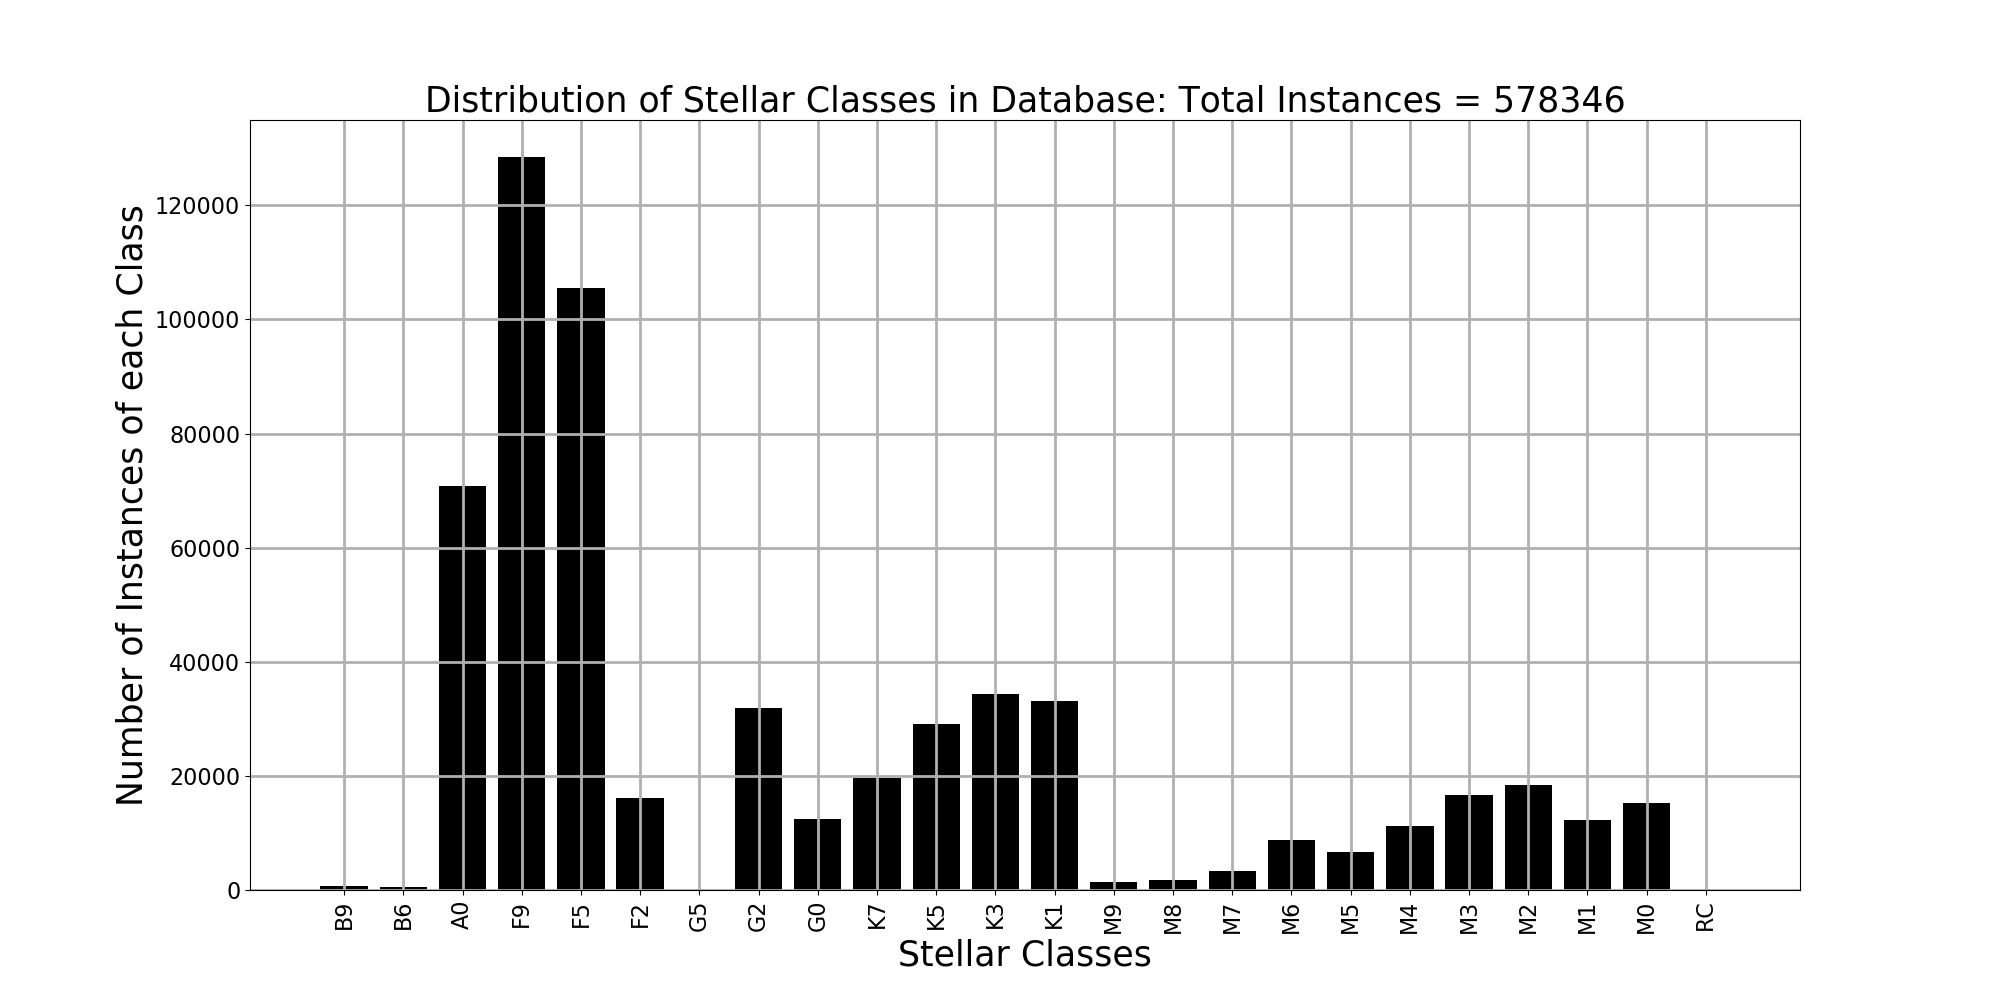
\includegraphics[width = 2.9in]{Distribution_S.png} %51
            \caption{Distribution of data.}
            \label{fig:dist1}
        \end{figure}

    \end{columns}
  \end{block}



\end{frame}

\subsection{Data pre-processing}
\begin{frame}
\frametitle{Data pre-processing}

\begin{itemize}
\item The flux is scaled from 0 to 1.
\item Each stellar spectrum in the dataset collected different amounts of flux measurements.
\item Problems for Feature Matrix (next slide)
	\begin{itemize}
		\item An average number of flux measurements is computed using the first 5,000 spectra. 
		\item Used to fit each spectrum to a standardized number of flux measurements.
		\item Average number of flux measurements is 3,834.
		\item Wavelength Fitting
		\item Redshift
	\end{itemize}

\end{itemize}
\end{frame}

\subsection{Feature Matrix}
\begin{frame}
\frametitle{Feature Matrix}
  \begin{block}

    \begin{columns}[t]
      \column{.45\textwidth} % Left column and width
\vspace{-0.5cm}
	
\begin{table}
        \centering
        %\Large
        \caption{Example of the feature matrix}
        \label{tab:feature-matrix}
        \resizebox{2.8in}{!}{
        \def\arraystretch{1.2}
\begin{tabular}{|c|c|c|c|c|}
\hline
           & \begin{tabular}[c]{@{}c@{}}Wavelength:\\ 3,807.15 $\mathring{A}$\end{tabular} & \begin{tabular}[c]{@{}c@{}}Wavelength:\\ 3,808.03 $\mathring{A}$\end{tabular} & \begin{tabular}[c]{@{}c@{}}Wavelength:\\ 3,808.90 $\mathring{A}$\end{tabular} & \begin{tabular}[c]{@{}c@{}}Wavelength:\\ 3,810.66 $\mathring{A}$\end{tabular} \\ \hline
Spectrum 1 & Flux                                                     & Flux                                                      & Flux                                                       & Flux                                                       \\ \hline
Spectrum 2 & Flux                                                       & Flux                                                      & Flux                                                       & Flux                                                       \\ \hline
\end{tabular}}
\end{table}
      \column{.5\textwidth} % Right column and width

\vspace{-0.8cm}

        % Example of redshift in the feature matrix
        \begin{table}
        
        \centering
        %\Large
        \caption{Example of the feature matrix that has redshifted data}
        \label{tab:example}
        \resizebox{2.8in}{!}{
                \def\arraystretch{1.2}
            \begin{tabular}{|c|c|c|c|c|c|}

            \hline 
            \begin{tabular}[c]{@{}l@{}}Star \\ Class\end{tabular} & \begin{tabular}[c]{@{}l@{}}Wavelength: \\ 6,560.8 $\mathring{A}$\end{tabular} & \begin{tabular}[c]{@{}l@{}}Wavelength: \\ 6,561.8 $\mathring{A}$\end{tabular} & \begin{tabular}[c]{@{}l@{}}Wavelength: \\ 6,562.8 $\mathring{A}$\end{tabular} & \begin{tabular}[c]{@{}l@{}}Wavelength: \\ 6,563.8 $\mathring{A}$\end{tabular} & \begin{tabular}[c]{@{}l@{}}Wavelength: \\ 6,564.8 $\mathring{A}$\end{tabular}
            \\ \hline
                A0 & & H$\alpha$ & & & \\ \hline
                A0 & H$\alpha$ & & & & \\ \hline
                A0 & & & H$\alpha$ & & \\ \hline
                A0 & & & & H$\alpha$ & \\ \hline
                A0 & & & & &  H$\alpha$\\ \hline
            \end{tabular}}
        \end{table}
        

    \end{columns}
  \end{block}
\end{frame}

\subsection{Classifier and Feature Selection Methods}

\begin{frame}
\frametitle{Classifier and Feature Selection Methods}

  \begin{block}

    \begin{columns}[t]
%\vspace{-0.8cm}
      \column{.5\textwidth} % Left column and width

Random Forest (RF)
	\begin{itemize}
	\item 10 Trees
	\item Other Authors report good accuracy \cite{YI}
	\item Weka demonstrated potential for good accuracy
	\end{itemize}

Support Vector Machine (SVM)
	\begin{itemize}
	\item Gaussian Kernel / RBF Kernel
	\item Authors report good accuracy \cite{Xing}
	\item Weka demonstrated potential for good accuracy
	\end{itemize}

      \column{.45\textwidth} % Right column and width
	
Chi Squared
\begin{itemize}
\item Chosen because of simplicity and low computational time.
\item Commonly used and is reliable \cite{Canedo}.
\end{itemize}

Fisher Score
\begin{itemize}
\item Chosen because of simplicity.
\item Performed well on other large astronomical datasets \cite{Zheng}.
\end{itemize}

    \end{columns}
  \end{block}

\end{frame}

\subsection{Results}
\begin{frame}
\frametitle{Results I}

\begin{table}[]
        \resizebox{4.5in}{!}{
                \def\arraystretch{1.2}
\begin{tabular}{|c|c|c|c|c|}
\hline
\multicolumn{5}{|c|}{Accuracy of Undersampled (12,584 Samples) Stellar Spectra}                         \\ \hline
K Best Features      & Redshift            & Rest             & Redshift            & Rest              \\ \hline
                     & \multicolumn{2}{c|}{Chi Squared + RF}  & \multicolumn{2}{c|}{Chi Squared + SVM}  \\ \hline
500                  & 83.59\%             & 88.24\%          & 40.41\%             & 41.27\%           \\ \hline
250                  & 80.92\%             & 86.72\%          & 38.73\%             & 39.59\%           \\ \hline
100                  & 80.81\%             & 86.17\%          & 33.60\%             & 35.69\%           \\ \hline
                     & \multicolumn{2}{c|}{Fisher Score + RF} & \multicolumn{2}{c|}{Fisher Score + SVM} \\ \hline
500                  & 84.95\%             & 87.40\%          & 64.66\%             & 63.81\%           \\ \hline
250                  & 83.45\%             & 86.27\%          & 64.44\%             & 61.02\%           \\ \hline
100                  & 82.00\%             & 83.46\%          & 66.51\%             & 56.06\%           \\ \hline
\end{tabular}}
\end{table}
\end{frame}

\begin{frame}
\frametitle{Results II}

\begin{table}[]
        \resizebox{5in}{!}{
                \def\arraystretch{1.2}
\begin{tabular}{|c|c|c|c|c|}
\hline
\multicolumn{5}{|c|}{Accuracy of Hybrid (367,004 Samples) Stellar Spectra}                  \\ \hline
K Best Features       & \multicolumn{2}{c|}{Chi Squared + RF} & \multicolumn{2}{c|}{Fisher Score + RF} \\ \hline
                      & Redshift           & Rest             & Redshift           & Rest              \\ \hline
500                   & 96.55\%            & 98.21\%          & 96.87\%            & 97.32\%           \\ \hline
250                   & 95.46\%            & 97.31\%          & 96.49\%            & 97.58\%           \\ \hline
100                   & 95.11\%            & 97.02\%          & 95.89\%            & 97.22\%           \\ \hline
\end{tabular}}
\end{table}
\end{frame}

\begin{frame}
\frametitle{Results III}

\begin{table}[]
        \resizebox{5in}{!}{
                \def\arraystretch{1.2}
\begin{tabular}{|c|c|c|}
\hline
\multicolumn{3}{|c|}{Execution Time (Seconds) for Hybrid (367,004 Samples) Rest Spectra with 500 Best Features} \\ \hline
                                     & Chi Squared + RF                   & Fisher Score + RF                   \\ \hline
Feature Selection                    & 17.48                              & 7.94 x $10^5$                       \\ \hline
Train                                & 109.06                             & 121.24                              \\ \hline
Test                                 & 0.74                               & 0.79                                \\ \hline
\end{tabular}}
\end{table}
\end{frame}

\section{Conclusions}
\begin{frame}
\begin{center}
\LARGE
Conclusions
\end{center}

\end{frame}

\begin{frame}
\frametitle{Conclusions}
\begin{itemize}
\item The entire spectrum is not necessary to obtain high accuracy.
\item Despite feature matrix complications, redshifted spectra can be accurately classified.
\end{itemize}
\end{frame}

\section{References}
\begin{frame}[allowframebreaks]{Reference}
    \bibliographystyle{plain}
    \bibliography{ref}
\end{frame}

\end{document}
